\chapter{Chaotic but regular recurrent influenza epidemics: from
  theory to observation}

%other title proposals
%\title{Chaotic dynamics with uniform phase in influenza
%  epidemics: from theory to observation}

Sébastien Ballesteros$^{1,*}$,
Lewi Stone$^{2}$,
Anton Camacho$^{1}$,
Elisabeta Vergu$^{3}$,
Bernard Cazelles$^{1,4}$

\vspace{2cm}

$^1$UMR 7625  (UPMC, ENS, AgroParisTech, CNRS), Ecole Normale
Supérieure, Unit of Eco-Evolutionary Mathematics,  46 rue d'Ulm,
F-75230 Paris Cedex 05, France. \\
$^2$Biomathematics Unit, Faculty of Life Sciences, Tel Aviv
University, Ramat Aviv 69978, Israel \\
$^3$~INRA, UR341 Mathématiques et Informatique Appliquées, F-78352 Jouy en Josas, France \\
$^4$~UMMISCO UMI 209 IRD-UPMC, F-93142 Bondy, France.

~\\
$^*$\textit{Corresponding author}:  \\
E-mail: sebastien.ballesteros@biologie.ens.fr

\section*{Abstract}


Human Influenza epidemics in temperate areas are characterised by a
relatively constant phase (despite influenza type or subtype
alternates) and highly variable amplitude. Influenza epidemics peaks
variability is currently explained by punctuated evolution of
influenza main antigen, higher peaks reflecting higher antigenic
changes.  We seek to determine to what extent gradual antigenic drift
alone (without perturbations induced by rare mutations with strong
antigenic effects) and therefore non-linear dynamics by itself can
induce Uniform Phase and Chaotic Amplitude (UPCA) dynamics. We present
a minimal model taking into account key processes of influenza
epidemiology and evolution. We show that this model presents UPCA
dynamics for a wide range of parameter value relevant for influenza
A. We then confirm the presence of UPCA dynamics in real data and
illustrate their robustness on a worldwide metapopulation model
including age structure, credible immigration rates and realistic
infectious time distribution. Finally, we argue that chaotic dynamics
with uniform phase should be the baseline scenario to consider when
trying to interpreter influenza epidemics size variability.  Influenza
UPCA dynamics therefore sets fundamental limits to the predictability
of future epidemics sizes in addition to evolutionary contingency.

~ \\
\textit{Keywords}: \\
Influenza, Gradual Antigenic Drift, Chaos, UPCA Dynamics, State-Space
Model, Particle Filter.

\section{Introduction}
\label{sec:introduction}

Interpandemic human influenza occurs annually in most temperate
climatic zones of the world with epidemics that peak in the cold
winter months. These outbreaks have been documented in the scientific
literature in records that extend back to at least 1650
\citep{Potter2001}, making it an exceptional example of a persisting
recurrent disease.  Being a respiratory infection, and highly
infective at that, influenza spreads from person to person in the form
of virus aerosol particles, and has the ability to propagate rapidly
through human populations. Average epidemics may have attack rates of
the order of 10-20 \% in cities but in certain susceptible populations
(school-children, nursing homes) the proportion of infecteds may reach
40-50 \% of the population \citep{Cox2000a}.  Influenza is thus a source
of considerable human morbidity and mortality, reaching some 250,000
to 500,000 deaths per year globally, and clearly exacting a large
overall economic toll on society.

There is still much controversy in identifying the seasonal drivers
that generate annual influenza oscillations, and the processes that
give rise to their large variability \citep{Finkelman2007}. These are
in fact outstanding problems of influenza research today, and are
addressed in detail from a modeling perspective here. As is well known
from the many studies of childhood infectious diseases, a necessary
requirement for the generation of recurrent epidemics is a sufficient
and continuous source of new susceptible individuals arising in the
population; enough to fuel each new outbreak. In the classical 1977
experiments of \citet{Potter1977} and \citet{Gill1977}, it was
established that although hosts infected with influenza gain immunity,
ultimately they may become susceptible once again and reinfected due
to the rapidly evolving nature of the influenza virus.  Positive
selection exerted by the host immune system, leads to a continual
antigenic drift of the influenza virus's glycoproteins, particularly
the main antigen hemagglutinin (HA), thus allowing the virus to
eventually evade the immune system.  The process of antigenic drift
thereby creates an important renewed source of susceptible
individuals.  Evolutionary forces are thus considered to be of
tremendous importance in shaping complex recurrent patterns of
infectious diseases \citep{Cobey2008}, and are the reasons why
influenza is regarded as ``an invariable disease caused by a variable
virus'' \citep{Potter2001}.

Recently, new theoretical developments along with recent data,
analyzed by phylogenetic and coalescent based approaches
\citep{Smith2004, Koelle2006, Wolf2006, Rambaut2008} have revealed
that the evolution of influenza A H3N2 main antigen (HA) is punctuated
with discrete antigenic clusters jumps. Epochal evolution,
materialised by sudden change of pathogens either due to mutations or
re-assortments can have large epidemiological impacts. Punctuated
immune escape therefore offers an intuitive explanation to the time
series of Human Influenza epidemics in temperate areas. Within the
scope of epochal evolution higher peaks can reflect higher antigenic
changes \citep{Koelle2006}.

The recent emphasis on punctuated immune escape has been the source of
important discussions with some authors rejecting epochal evolution in
favour of a more gradual immune escape pattern \citep{Shih2007,
  Suzuki2008, Ballesteros2009}. In this paper we add new arguments to
the debate by focusing on the information that can be inferred from
influenza incidence time series at the population level.  We seek to
contrast ``an extrinsic view'' \citep{Cobey2008} of influenza dynamics
where antigenic cluster transitions induce epidemic amplitude
variability and higher peaks reflect larger antigenic changes, with
``an intrinsic view'' of purely gradual evolution where epidemic size
variability can only result from the internal nonlinear dynamics of
the system.

Our modeling effort focuses on the dynamics of influenza A, given that
of the different influenza types, A contributes most to human disease
burden.  We begin by formulating a minimal mathematical model that
characterizes its dynamics as having Uniform Phase, or regular
periodicity in rhythm, together with epidemic peaks having irregular
Chaotic Amplitudes; a phenomenon referred to here in short as UPCA.
We confront our modeling results with time series data and argue that
UPCA dynamics should be the baseline scenario to consider when trying
to interpret the complex population dynamics of recurrent influenza
epidemics.  As seen in Figure~\ref{fig:attractor}, long-term influenza
time series from both France and Israel make evident that the UPCA
dynamics are a characteristic feature.  To our knowledge, no previous
deterministic modeling attempts of single or multi-strain dynamics
have been able to reproduce the fundamental characteristics of UPCA
which are inherent in many observed influenza time series.  These
findings around the nonlinear nature of the mechanisms of transmission
highlight that in addition to evolutionary contingency, diseases as
influenza have fundamental limits to the predictability of future
epidemic sizes.


\begin{figure}[htbp]
  \center
  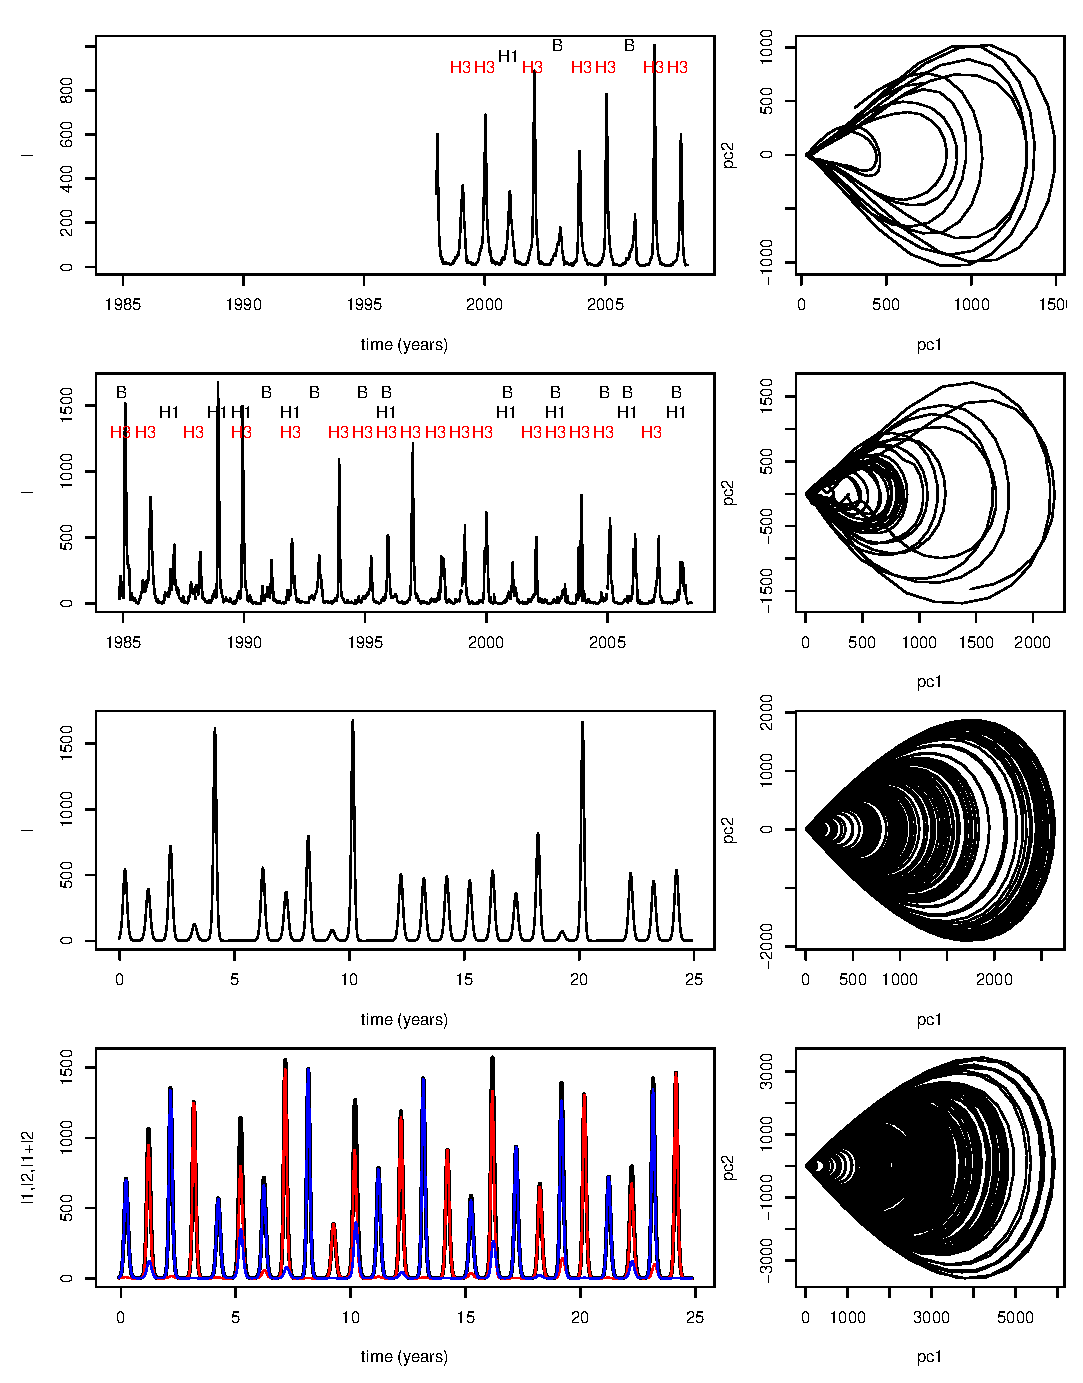
\includegraphics[width= 0.8 \linewidth]{texte/article2/graph/all_reconstructed_bernard_theo.eps}
  \caption{Weekly incidence rates for Influenza Like Illness per 100
    000 hosts in Israel (first line) and Ile de France (French
    administrative region including Paris and its surrounding area;
    second line). Data from Israel have been corrected to take into
    account a reporting rate of 1/3.
    Other lines: Typical weekly incidence rate
    simulated with the deterministic single subtype $SIRS$ model (third
    line) and the deterministic two-subtype model (fourth line).
    % 
    Right graphs are phase state representation (after a principal
    component analysis) with embedding realised by the method of delay
    where $pc1$ and $pc2p$ are the two first components.
    % 
    Parameters: third line: maximum likelihood estimate for Ile de France
    ($R_0=1.65$, $1/\nu=2.47$ days$^{-1}$, $e=0.104$) with $1/g=7$
    years$^{-1}$ and $\eta=10^{-6.7}$) ; fourth lines: theoretical
    parameter set with $e=0.35$, $1/g=15$ years$^{-1}$, $1/q=6$
    months$^{-1}$ and $\eta=10^{-6}$.
    % 
    Additional trajectories are provided in Supporting Information.}
  \label{fig:attractor}
\end{figure}


\section{Theory}
\label{sec:theory}

\subsection{A minimal model for influenza A}
\label{sec:model}


We consider a minimal model that takes into account three key
processes of influenza dynamics in temperate areas: seasonal forcing,
external reintroductions and antigenic drift \citep{Nelson2007}.

The importance of the role of seasonal forcing has long been
acknowledged and is best observed by comparing influenza seasonal
patterns along a latitude gradient: the seasonal patterns range from
marked seasonal winter activity centred around January in the Northern
hemisphere, to uniform circulation throughout the year in the Tropics
and again, strong winter epidemics center around July in the Southern
hemisphere \citep{Viboud2006}. Climatic triggers appear to be involved
\citep{Alonso2007a} and influenza transmission has been reported to be
controlled by absolute humidity \citep{Shaman2009}.  However, a
precise understanding of what drives seasonal influenza trends has not
yet been achieved \citep{Lipsitch2009}. A further complication may be
linked to the fact that although seasonality may appear to dominate,
its intensity might not necessarily be strong if there is dynamical
resonance as speculated in \citet{Dushoff2004}.

Related to the seasonal patterns of influenza, recent developments
made possible through the availability of large genetic data sets,
have revealed that global influenza is a source-sink system, with the
tropics constantly reseeding the temperate areas \citep{Rambaut2008,
  Russell2008}. The antigenic change observed in temperate populations
seems to be a secondary effect of strong selection within, and largely
unidirectional flow from the source population where sustainable year
long transmissibility favours successful antigenic changes. This
advance renders migration and re-introduction of influenza key
processes to consider when studying the dynamics of influenza across
seasons in temperate areas.

As already mentioned, the punctuated versus gradual nature of
antigenic drift is currently highly controversial
\citep{Ballesteros2009}. Previous studies have derived estimates of
the rate of antigenic drift. \citet{Potter1977} found that the
probability of reinfection increases linearly with time since last
infection due to an average antigenic drift rate estimated to be
1/19.5 years$^{-1}$ \citep{Pease1987}.  Statistical inference methods,
as used in \citet{Finkenstaedt2005}, have resulted in estimates of the
gradual component equal to 1/13 years$^{-1}$ with a model accounting
only for purely gradual antigenic drift and to 1/23.3 years$^{-1}$ in
a model that allows for punctuated evolution and discrete antigenic
change.

Taking into account these three key processes results in the model of
equation~\eqref{eq:sirs}, schematically described in
Fig.~\ref{fig:sirs} and detailed in Methods.

\begin{figure}[htbp]
  \center
  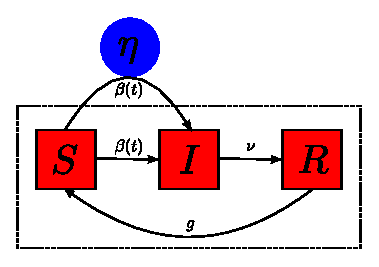
\includegraphics[width= 0.3 \linewidth]{texte/article2/graph/sirs.eps}
  \caption{A minimal model for a given subtype of influenza A: $S$ is
    the number of susceptible hosts, $I$ the number of infectious
    hosts and $R$ the number of recovered and temporary immunised
    hosts. $\beta(t)$ is the transmission rate taking into account
    seasonality, $\nu$ the recovery rate, $g$ the antigenic drift rate
    (due to viral evolution) and $\eta$ is the contribution of
    infectious hosts from external regions to the force of infection.}
  \label{fig:sirs}
\end{figure}

The first model with a single sub-type can be easily generalized for
many co-circulating subtypes assuming that subtypes only interact via
a temporary period of full cross-immunity as suggested by
\citet{Webster1992}.  Such a model with two subtypes, representing for
instance the co-circulation of H3N2 and H1N1 influenza A subtypes as
has been the case since 1977 \citep{Earn2002}, was analyzed (see
Methods and Supporting information).

In order to study the dynamics of the models of eq~\eqref{eq:sirs}
and~\eqref{eq:HB}, we make use of two sets of parameters. One consists
of parameters commonly adopted in theoretical papers (\textit{e.g.}
\citet{Koelle2006, Ferguson2003, Goekaydin2007}) and the other
consists of more direct estimates of parameters from household studies
(\textit{e.g.} \citet{Cauchemez2004, Lavenu2004}). Both parameter sets
are listed in Table~\ref{tab:param}.  The remaining parameters ($e$,
$g$ and $\eta$) are considered as bifurcation parameters.

\begin{table}[htb]
  \center
  \begin{tabular}{|l|l|l|}
    \hline
    Parameters & Theoretical & Empirical\\
    \hline
    $\nu$ (recovery rate) & $1/8$ days$^{-1}$ \citep{Koelle2006} & $1/2.77$ days$^{-1}$ \citep{Lavenu2004} \\
    \hline	
    $R_0$ ($\beta=R_0 \nu$) & $5$ \citep{Koelle2006} & $2.66$ \citep{Lavenu2004} \\
    \hline		
  \end{tabular}
  \caption{Parameter values}
  \label{tab:param}
\end{table}

\subsection{UPCA dynamics in influenza epidemics}
\label{sec:res_upca}

As mentioned above, UPCA dynamics is a good candidate to explain
influenza incidence time series in the absence of rare mutation with
strong antigenic effects. The uniform phase characterizes the regular
annual outbreak, while the chaotic amplitudes of the number of
infectives characterizes the irregular peaks of the epidemics from
year to year. In the following, we will shortly show that the simple
models outlined above (eq.~\eqref{eq:sirs} and~\eqref{eq:HB})
naturally generate UPCA dynamics.

UPCA dynamics was first introduced in theoretical ecology by
\citet{Blasius1999} in the context of ecological foodwebs. For
epidemiological systems represented by the classical forced $SIR$
models, we have found that it is difficult, if not impossible, to
locate parameter regimes in which outbreaks occur regularly each
year. For instance, for SIR systems, there are numerous years without
epidemics \citep{Stone2007a, Olinky2008}, and this appears to be an
intrinsic feature of these models.

In contrast, the $SIRS$ models with immigration (eq.~\eqref{eq:sirs}
and~\eqref{eq:HB}), and especially the version where multiple subtypes
co-circulate, prove to be better candidates for UPCA dynamics because
the presence of a higher rate of susceptible renewal resulting from
antigenic drift and external infections both facilitates epidemic
``re-birth'' after large events of susceptible depletion.
Figure~\ref{fig:attractor} and Supporting Information display typical
model realizations of Eqns.~\eqref{eq:sirs} and~\eqref{eq:HB} and make
clear the occurrence of strong annual outbreaks, although their
intensity is quite different, and in fact chaotic, from year to year.

To assess whether UPCA dynamics is a commonplace or a pathological
feature of the model, its dynamics have been scanned over a large
range of parameter space. That UPCA dynamics is chaotic, means that it
can be detected by checking for a positive first Lyapunov exponent
following the algorithm of \citet{Wolf1985}. Phase regularity was
identified by demanding than 95\% of the inter-peak intervals ranged
between 0.7 and 1.3 years (other measures for phase stability do not
significantly alter the results). To ensure that we do not select
trajectories with several years between two epidemic peaks, we
retained only time series having all maxima with amplitudes that are
higher than 5\% of the endemic equilibrium in the absence of seasonal
forcing. This value (5\%) was found appropriate to allow years with
very low peaks (akin to the refractory period reported by
\citet{Koelle2006} after antigenic cluster transitions) but
sufficiently high to ensure that the following year is characterized
by with a significant peak (in accord with data).

Figure~\ref{fig:main2} reveals the results of the bifurcation analysis
for both the one subtype and two subtype models. In all cases, UPCA
dynamics can be found in wide areas of realistic parameter values for
influenza. In particular, UPCA dynamics are possible for antigenic
drift values compatible with estimates of \citet{Finkenstaedt2005} and
\citep{Pease1987} who report gradual antigenic drift rates ranging
from 1/13 to 1/25 years$^{-1}$.

As can be seen in figure~\ref{fig:attractor} and Supporting
Information it is striking how the single subtype SIRS UPCA model is
able to produce patterns reminiscent of antigenic cluster transition,
(years with a significantly higher peak followed by a refractory
period of one year) with only purely gradual antigenic drift. Even
more surprising, the period in between those refractory period closely
matches the reported duration of antigenic cluster persistence ranging
for 1 to 8 years \citep{Smith2004}.

\begin{figure}[htbp]
  \center
  \includegraphics[width= 0.8 \linewidth]{texte/article2/graph/main2.eps}
  \caption{First Lyapunov exponent and parameters space where we
    expect UPCA dynamics (black contours). Top : single subtype model
    ; bottom: Two co-circulating subtypes model for an average 6
    months period of temporary full cross-immunity.  Left graphs are
    for theoretical parameters values ($R_0=5$ ; $1/\nu=8$ days ;
    $\eta=1.10^{-6}$) ; Right graphs are for empirical parameters
    values ($R_0=2.66$ ; $1/\nu=2.77$ days ;
    $\eta=1.10^{-7}$. Supplementary figure in Supporting Information
    provides the periods bifurcations.}
  \label{fig:main2}
\end{figure}


\section{Corroborations from observations}
\label{sec:confirmation}

First we qualitatively compare the time series and the attractors of
the observation and simulation of the models. Figure
\ref{fig:attractor} (right part) presents a phase space representation
of the ILI data from Israel and Ile de France as well as comparisons
with two dimensional projections of the strange attractors of the
model of eq~\eqref{eq:sirs} and~\eqref{eq:HB} (two subtype case). All
these graphs show general good agreement between the theoretical and
the reconstructed phase space representation.

To confirm these qualitative results, we have compared the UPCA model
to real data, by implementing a stochastic version of
eq~\eqref{eq:sirs} (see Supporting Information) and using maximum
likelihood identification. Parameter inference was achieved with an
implementation of maximum likelihood via iterated filtering (MIF) as
described in \citet{Ionides2006} and \citet{Breto2009} (see Supporting
Information).
The results of the inference procedure are depicted in Supporting
Information. The transmission and antigenic drift rates were difficult
to estimate and appeared to be strongly correlated as can be seen in
Supporting Information. 

%Indeed, we found that a given level of
%infective with the same overall qualitative dynamics could be obtained
%by modifying $\beta_0$, $g$ being fixed or by modifying $g$ while
%keeping $\beta_0$ constant..
%This correlation is a cause of concern for
%studies estimating the basic reproductive number of influenza. based on
%the first growing parts of the epidemic curve and therefore neglecting
%the effect of antigenic drift (\textit{e.g.} \citet{Chowell2008a}). If
%such studies provide valuable insights to the value of $R$, the link
%to $R_0$ is difficult to made \citep{McVernon2007, Mathews2009} and 

We then examine to what extent the inferred parameters (see Supporting
Information) were compatible with UPCA dynamics. Due to the
uncertainty of the antigenic drift rate and given the difficulty to
directly insert the external infection parameter from the stochastic
model to the deterministic model (eq~\eqref{eq:sirs}) we considered
$g$ and $\eta$ as bifurcation parameters and fixed the other
parameters to their maximum likelihood values.

Figure \ref{fig:eta_best_fit2} reveals that these parameter inferred
for ILI data of Ile de France region are within the UPCA area of the
deterministic model for a large range of $g$ and $\eta$ values. All
these results corroborate the interest of the UPCA dynamics in
influenza epidemics.

% Moreover it is important to specify that the simulated time series
% presented Fig. 1 and Fig. S have been obtained with the parameter
% inferred from ILI data of region Ile de France.

\begin{figure}[htbp]
  \center
  \includegraphics[width= 0.8 \linewidth]{texte/article2/graph/eta_best_fit2_g11.eps}
  \caption{One dimensional and two dimensional bifurcation diagram for
    external infectious hosts parameter ($\eta$) and antigenic drift
    rate ($g$). Other parameters are fixed at their maximum likelihood
    estimate from Supporting Information ($R_0=1.65$, $1/\nu=2.47$
    days$^{-1}$, $e=0.104$). Supplementary Information provides the
    periods bifurcations.  }
  \label{fig:eta_best_fit2}
\end{figure}

\section{Robustness}
\label{sec:robustness}

Due to the growing recognition of the punctuated nature of immune
escape \citep{Cobey2008} we have checked to what extent UPCA dynamics
are robust to perturbations due to rare mutation with higher than
usual antigenic effects. For this purpose, we have generalised the
model of eq.~\eqref{eq:sirs} so that at random times, these
perturbations are applied by transferring a percentage $x \in [0,1]$
of recovered hosts into the susceptible compartment. In order to
quantify the magnitude of $x$ we have used the ratio of the maximum
number of infected hosts in the presence of perturbations over the
maximum number of infected hosts for a typical unperturbed UPCA
trajectory. This ratio is plotted in figure~\ref{fig:pert} (right
panel).  Contrasting this ratio to the ILI data, enabled us to set a
maximum boundary for $x$ at 0.07.  This value is in accord with
\citet{Finkenstaedt2005} who estimated from French ILI data $x$
values smaller than 7\% (53\% of the estimates $\leq 2\%$ ; 26.7\%
between 2 and 5 \% and 20\% between 5 and 7\%).
Figure~\ref{fig:pert} reveal that UPCA dynamics is robust to such
perturbations, the transient being shorts.  As suggested by
\citep{Koelle2006}, we also notice that punctuated immune escape can
induce higher peaks followed by refractory periods. However the
occurrence of such a pattern strongly depends on the time of the
perturbation and is not systematic.

\begin{figure}[htp]
  \center
    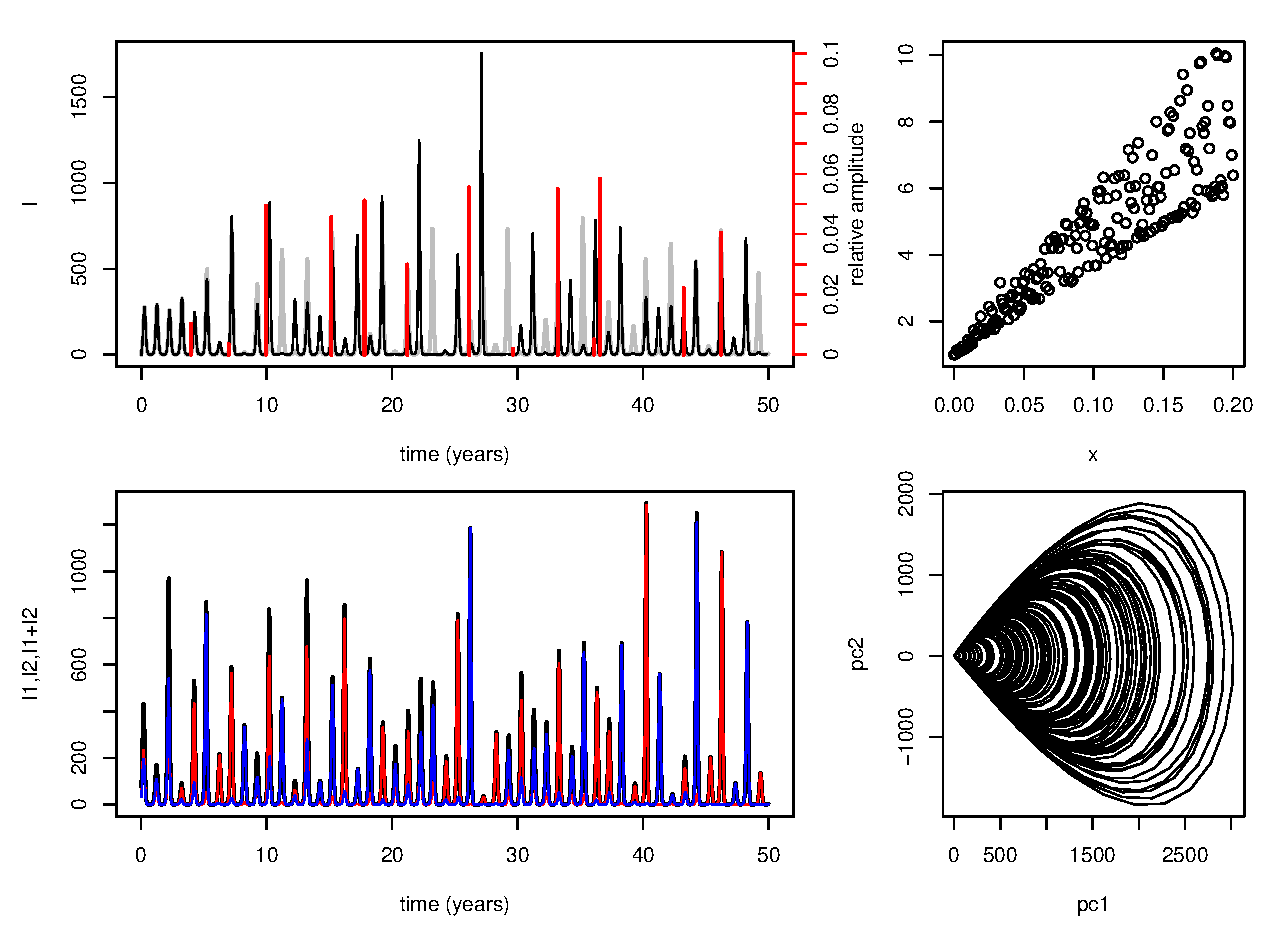
\includegraphics[width= 0.8 \linewidth]{texte/article2/graph/pert.eps}
    \caption{Robustness of UPCA dynamics.  %
      First line: effect of environmental stochasticity. Left panel:
      Gray line represents an unperturbed UPCA trajectory for
      parameters $R_0=1.65$, $1/\nu=2.47$ days$^{-1}$, $1/g=11$
      years$^{-1}$, $e=0.104$, $\eta=10^{-7}$. The same perturbed
      trajectory is plotted in black. Perturbation times and amplitude
      ($x$, reported on right axis) are indicated by red vertical
      lines. Perturbation times are sampled from a Gaussian
      distribution with mean=3.3 and sd=1.9 corresponding to values of
      antigenic cluster succession reported by
      \citet{Smith2004}. Perturbation intensity ($x$) are sampled from
      an Uniform distribution defined on the interval $[0, 0.07]$. Right panel: ratio of the
      maximum number of infected host in the presence of perturbations
      over the maximum number of infected host for the
      same unperturbed trajectory as a function of $x$.
      % 
      Second line: A typical realization of the stochastic 2 subtypes
      metapopulation model for Paris and the associated phase state
      representation (after a principal component analysis where $pc1$
      and $pc2$ are the 2 first components) with embedding realised by
      the method of delay obtained with the empirical parameter
      set. Other parameter are $1/g=25$ years$^{-1}$, $1/q=6$
      months$^{-1}$, $1/ \gamma=1.5$ days$^{-1}$). Seasonal forcing
      ($e=0.2$) for Northern and Southern hemisphere cities are in
      phase opposition and tropics do not present seasonality (see
      Supporting Information) .}
  \label{fig:pert}
\end{figure}

The robustness of the UPCA dynamics was also tested by increasing the
realism of the model in various ways.  First, we constructed a
stochastic metapopulation version of the model of eq~\eqref{eq:HB}
with realistic inter-city migration based on transportation data flow
from 52 major cities over the world published in \citet{Grais2003}
(see Supporting Information). Second, more realistic infection time
distributions were employed by incorporating an exposed class ($E$)
and by using Erlang distributions for sojourn times in exposed and
infectious states instead of exponential. Third, three age classes
were considered using \citet{Wallinga2006} data from social contacts
to estimate age-specific transmission parameters. The full model is
detailed in Supporting Information.  Figure~\ref{fig:pert} and
Supporting Information reveal the robustness of UPCA dynamics that
appears little affected by demographic stochasticity, metapopulation
dynamics, age structure and non exponential infected time
distribution.


\section{Discussion}
\label{sec:discussion}

%1-
The studies of \citet{Smith2004, Koelle2006, Wolf2006, Shih2007} and
\citet{Suzuki2008} have generated controversies on the exact patterns
of influenza A antigenic evolution, potentially challenging the purely
gradual view expressed by \citet{Pease1987}.  At the epidemiological
level influenza epochal evolution has offered an intuitive explanation
to epidemics peaks variability observed in data.  Here, we have
illustrated that non-linear dynamics alone, under a purely gradual
antigenic evolution scenario can results in dynamics strikingly
similar both qualitatively and quantitatively to the one that are
expected under the punctuated immune escape scenario.  Care should
therefore be taken when considering that higher epidemic peaks
reflect punctually large antigenic changes.

UPCA dynamics also offers a parsimonious explanation to the previously
unexplained fact that influenza most severe seasons are not always
associated with antigenic novelty, but with antigenically similar
strains returning for several consecutive seasons. For instance,
\citet{Viboud2006b} cite the striking examples of the 1989-1990
epidemic in the UK (A/England/89 (H3N2) strain) or the 1999-2000
epidemic in the US (A/Sydney/97 (H3N2) strain).

%2-perspective & inference
If our results are not sufficient to reject punctuated immune escape,
they raise important questions about the potential effect of antigenic
cluster transition at the epidemiological level. In particular, given
the increasing recognition of functional constraint at the genomic
scale \citep{Rambaut2008, Du2008} immune escape advantage due to
antigenic cluster transition could be largely balanced by an
associated fitness cost \citep{Holmes2005}. Such functional trade-off
between antigenic escape and intrinsic fitness could easily explain
the good agreement with data obtained with our simple model neglecting
antigenic clusters.  This could also explain why \citet{Chowell2007a}
did not detect higher transmissibility when new antigenic clusters of
influenza A/H3N2 strains emerged in their estimates of the
reproduction numbers of seasonal influenza epidemics spanning over
three decades in the United States, France, and Australia.

The statistical framework used in this paper and developed in
\citet{Ionides2006} and \citet{Breto2009} provides a method to
determine to what extent a model with variable antigenic drift rate
(representing punctuated immune escape) is able to outperform the
minimal model presented here. We are currently investigating this
direction with the class of stochastic processes with stochastic rate
introduced in \citet{Breto2009}. Adding noise to gradual antigenic
drift parameter will allow to access to the variability of the
antigenic drift rate in a full likelihood based approach thus allowing
for model selection.  The same framework could also be used to assess
the highly debated existence of hetero subtypic partial cross-immunity
for influenza \citep{Epstein2006}.

%3-pandemics
In the context of the spread of the new animal origin H1N1 subtype, it
is important to have an appropriate, pertinent and tractable model to
describe both the initial conditions at the beginning of the pandemics
(resulting from the co-circulation of H3N2 and H1N1 subtypes since
1977 \citep{Earn2002}) and the competition between the three subtypes.
Such a description is of great interest for predicting the outcome of
the invasion of new influenza subtypes within a realistic ecological
context.  For instance the fact that the last epidemic season of the
A/H2N2 era was consistently lower in North America than elsewhere is
suspected to have been a key determinant to explain that the first
pandemic season of A/H3N2 influenza virus (1968/1969) resulted in
significant mortality in the United States, but that it was the second
pandemic season of A/H3N2 influenza virus (1969/1970) that caused the
majority of deaths in Europe and Asia \citep{Viboud2005}.  We think
that our coupled SIRS UPCA models have the characteristics to be such
an adapted and pertinent model for this task.

%4- ouverture et generalisation
As a last point, influenza UPCA dynamics could provide an example of
non-linear dynamics at work in nature setting limits to our ability to
predict future epidemics sizes in addition to evolutionary
contingency. It remains to be seen to what extent UPCA dynamics could
be a characteristic of other diseases. Norovirus whose phylodynamics
appears to be close to influenza \citep{Lopman2008} appears to be a
good candidate for further investigations.

%inclure...
%a inclure ou pas ?-
%\citet{Dushoff2004} dynamical resonance unclear
%comparaison des variances
%to add:
%a perturbated limit cycle floquet theory small perturbation 




\section*{Methods}

We briefly present the data, the models and the methods used here and
provide the technical details in the Supporting information.

We have used both daily incidence of Influenza Like Illness (ILI) of
Israel (REFERENCE FROM Lewi) and weekly incidence rates for region Ile
de France (Paris and its surrounding area) from the French Sentinelles
network (http://websenti.b3e.jussieu.fr/sentiweb/). The data are
plotted in figure \ref{fig:attractor}. The French data set was
selected for comparison purposes given the previous analysis of
\citet{Finkenstaedt2005}. Moreover, the French Sentinelles surveillance
system provide well described data spanning over 25 years.
 

Phase space representation of the data (e.g. \citet{Kantz2003}) was
achieved with the method of delay with an embedding dimension
determined by the false nearest neighbours method as implemented in
the \textit{tisean} package \citep{Kantz2003}. In case of the method
of delay, principal components analysis was then used to project the
reconstructed attractor on two dimensions.  Analytic signal and the
Hilbert transform were found to give similar results (results not
shown).

The first minimal model used takes into account three key processes of
influenza dynamics in temperate areas: seasonal forcing, external
reintroductions and antigenic drift. It only considers purely gradual
antigenic drift, in the same way as \citet{Pease1987}. For this model
of a given subtype of influenza A, the host population is divided into
three classes. As is usual, we set $S$ as the number of susceptible
hosts, $I$ the number of infectious hosts and $R$ the number of
recovered hosts with temporary immunity. Upon contact with an infected
host, susceptibles move to the infected class at a rate that is
determined by the parameter $\beta(t)$. The contact rate $\beta(t)$
also takes into account seasonality through annual sinusoidal
forcing. After a period determined by the rate $\nu$, usually several
days, infected hosts recover from influenza and for a period are
immune from further infection. However, due to antigenic drift of the
influenza virus which occurs continuously at a rate $g$, the immunity
fades and recovered individuals become susceptible once more, thereby
closing the SIRS loop (see figure~\ref{fig:sirs},
eq~\eqref{eq:sirs}). The constant force of infection term $\eta$,
represents the contribution of infected hosts from external regions.

\begin{footnotesize}
  \begin{align}
    \label{eq:sirs}
    \frac{dS}{dt} &=-\beta(t) \frac{S}{N} (I+\eta) +g R \\
    \frac{dI}{dt} &= \beta(t)  \frac{S}{N} (I+\eta) -\nu I  \notag \\
    \frac{dR}{dt} &= \nu I -g R \notag
  \end{align}
\end{footnotesize}
with $\beta(t)=\beta_0 (1+e \cos(2 \pi t))$.

The above model may easily be generalized for many co-circulating
subtypes assuming that subtypes only interact via a temporary period
of full cross-immunity as suggested by \citet{Webster1992} leading to
eq~\eqref{eq:HB} (Supporting Information provides a schematic
representation for the 2 subtypes case) . \citet{Ferguson2003} and
\citet{Tria2005} have shown that a temporary period of full
cross-immunity is necessary to restrict otherwise increasing strain
diversity in multi-strain models allowing for realistic antigenic
space in the absence of punctuated evolution. Its inclusion is
therefore needed in the purely gradual antigenic drift hypothesis.

\begin{footnotesize}
  \begin{align}
    \label{eq:HB}
    %% R
    \frac{dR_J}{dt} &= q Q_J - \sum_{k \notin J} \beta_k(t)
    \frac{R_{J}}{N} (I^k+\eta_k) -\sum_{k \in J} g_k R_{J} + \sum_{k
      \notin J} g_k
    R_{J \cup k } \\
%%
    %% I
    \frac{dI^k_{J \setminus k}}{dt} &= \beta_k(t) \frac{R_{J \setminus
        k}}{N} (I^k+\eta_k) - \nu I^k_{J \setminus k} -\sum_{m \in J
      \setminus k} g_m I^k_{J \setminus k} + \sum_{m \notin J
      \setminus k} g_m I^k_{(J \setminus k) \cup m}
    \notag \\
%%
    %% Q
    \frac{dQ_J}{dt} &= \sum_{k \in J} \nu I^k_{J \setminus k} - q Q_J
    -\sum_{k \in J} g_k Q_{J} + \sum_{k \notin J} g_k Q_{J \cup k }
    \notag
  \end{align}
\end{footnotesize}

with $I^k=\sum_{M \in J \setminus k} I^k_M$.

$I^k_{J\setminus k}$ are the hosts currently infected by subtypes $k$
resulting from infections from hosts who were immunized toward strain
belonging to the subset $J \setminus k$ ($J$ which does not contain
$k$). After recovery, infectious hosts $I^k_{J\setminus k}$ spend an
average time $1/q$ in the class $Q_J$ where they are ``invincible''
due to the temporary period of full cross-protection and then pass to
class $R_J$ where they are susceptible to every subtype not present in
subset $J$. $g_k$ is the gradual antigenic drift rate of subtype $k$.

As antigenic drift dominates susceptible renewal over demographic
processes, Eq~\eqref{eq:sirs} and~\eqref{eq:HB} do not include birth
and death process. Moreover their inclusion was found to have only
minor effects.

Eq. \eqref{eq:HB} was extended to a stochastic metapopulation model of
52 major cities over the world including 3 age classes. To increase
realism, an exposed period was added and exposed and infectious
classes were doubled to ensure that the exposed and infectious period
followed Erlang distributions.  Following \citet{Cooper2006a} it was
assumed that only exposed individuals traveled. The full model is
described in Supporting Information.

\section*{Acknowledgements}
This work was partially funded by the R\'egion Ile-de-France and the
“ANR-Agence Nationale de la Recherche – The French National Research
Agency” under the project ANR 05SEST01802 BIOSCOPE.


%%% Local Variables: 
%%% mode: latex
%%% TeX-master: "../../phD"
%%% End: 
